%\todo{RONALD - first draft by 30/May}

\subsection{Mechanisms and algorithms}
\todo{Peer Manager Theory - including flow diagram, pseudo-code if needed, whatever explain how it works}



\subsection{Implementation}
%{\it including how it has been implemented and specifications of APIs}

The Peer Manager component has been developed by following a three layered approach, where each layer leverages the basic services offered by the level below and composes them for producing higher-level services. This structure is shown in Figure~\ref{fig:pm-component-layers} and each layer will be further described in the rest of this section. 

\begin{figure}[htbp]
\centering
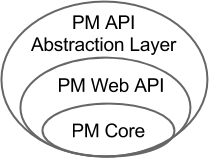
\includegraphics[width=0.4\textwidth]{figures/pm-component-layers.png}
\caption{Implementation layers of the Peer Manager}
\label{fig:pm-component-layers}
\end{figure}


\subsubsection{Peer Manager Core}
Its main purpose is to provide a privacy aware semantic storage for the SmartSociety Platform. This layer is implemented using Java, along with common data access frameworks like Spring and Hibernate.
While these technologies represent previous work from the University of Trento, the SmartSociety (through the work documented in D1.1, D4.1 and D4.2) has created the Knowledge Model used for representing peers, users, profiles (i.e. personal information) and more generally managing the information for running an HDA-CAS.

No major changes have been done to the models or structures of the Peer Manager during the first half of year three (so the research reported in previous deliverables still holds) but efforts to update these models to its final version for the SmartSociety project will start on the second part of year three (as T1.4 restarts) and will have its results reported in D1.3. It is not expected that radical changes to the models and structures are done in this revision so the underlying code and the exposes calls would probably receive only minor revisions as a result of this. 

\subsubsection{Peer Manager Web API} \label{ssec:pm-web-api}
This layer takes the Java classes that implement the Peer Manager Core and wraps them in HTTP API calls. 
No great changes, save for small adjustments and bug fixes were introduced to this layer in year three. As such the same information from deliverable D4.2 largely applies to this layer.
API specification for this layer may be found in the Appendix~\ref{sec:pm-web-api-detail}.

\todo{Content describing the purpose of this layer and the technologies used to implement it will be added to this section for the final version of this document}

\subsubsection{Peer Manager abstraction layer API} \label{ssec:pm-abs-api}
This is a new component being developed specifically for the SmartSociety project and as such all code belonging to this layer will be open sourced. API Specifications for this layer may be found in the Appendix~\ref{sec:pm-abs-api-detail}.

\todo{Content describing the purpose of this layer and the technologies used to implement it will be added to this section for the final version of this document}

\subsubsection{Integration with PPL policy language}
\todo{This content is forthcoming}